\subsection{question 4: Model Expansion and Generalization}
\subsubsection{Model Test Results}
\begin{figure}[bt!]
    \centering
    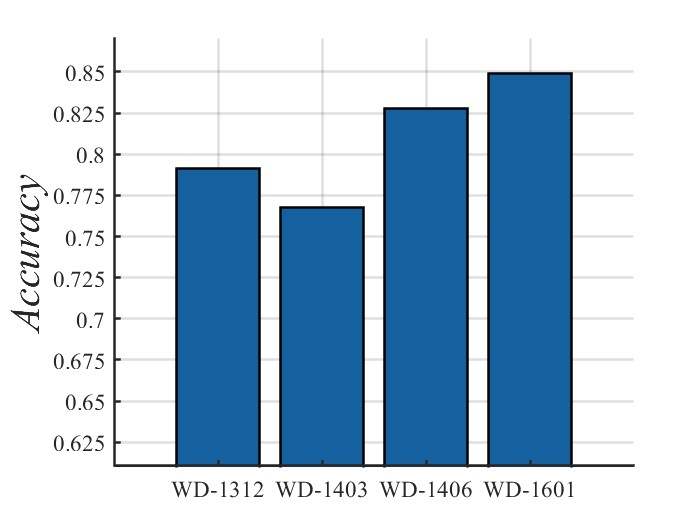
\includegraphics[width=0.5\linewidth]{figure/lstm4.png}
    \caption{\centering Prediction in some matches}
    \label{fig:lstm4}
\end{figure}
As stated before our model training has been based on all the data provided by the problem, so all our previous prediction results are for all matches. In Figure \ref{fig:lstm4} we provide a set of partial results from the test set.\par
As shown in the graph, the prediction accuracy fluctuates from match to match, and we believe that this is due to fluctuations caused by differences in players, etc. from match to match. This again illustrates the importance of introducing player-targeted analysis. \par


\subsubsection{Model Expansion}
When predicting the outcome of a tennis match, it is important to realize that the outcome of the match is not only determined by factors such as the situation on the court, player errors, etc. but is also affected by a combination of factors. We believe that to build a comprehensive and reliable predictive model, a range of key variables must be considered. These variables are summarized as follows:
\begin{itemize}
    \item \textbf{Age of Athlete}\\
    It can be seen from the reference \cite{ref3} that as the age increases, the speed and explosive power of tennis players will reach their peak. It can also be seen from the diagrams excerpted from the Figure \ref{fig:ECAG} that athletes' physical abilities will gradually reach their peak as they grow older during adolescence. As we age, our physical capabilities also decline. When predictive modeling of athlete physical condition, relying solely on observed running distance during a game to predict physical condition would be a simplistic approach. Instead, a more comprehensive and objective assessment of an athlete's physical condition can be achieved by quantifying physical capabilities relative to their age.
    \begin{figure}[b!]
        \centering
        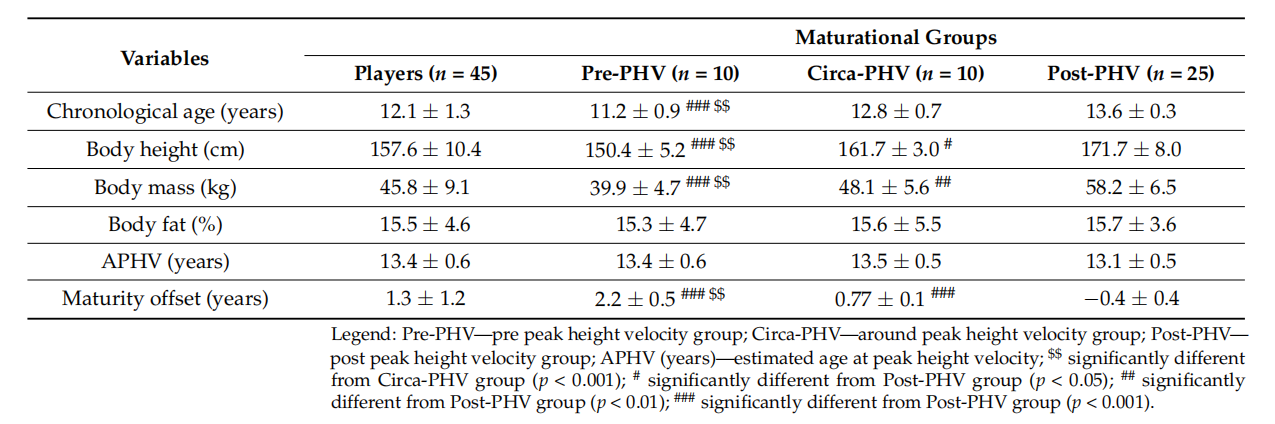
\includegraphics[width=0.75\linewidth]{figure/d021c08d7368ca795e638142b768207.png}
        \caption{\centering Extract Charts and Graphs}
        \label{fig:ECAG}
    \end{figure}

    
    \item  \textbf{Athlete Injuries and Illnesses}\\
    Based on the referenced document \cite{ref4}, it is clear that an athlete's injury status can significantly impact their performance. Injuries can profoundly affect technical aspects such as flexibility, speed, and strength. For instance, an injury to the lower extremities could result in reduced acceleration or impaired agility during directional changes. \\
    The repercussions of injuries are not limited to physiological aspects; they can also exert considerable psychological stress on athletes. Players dealing with injuries often face increased mental pressure during competitions, which can considerably impede their performance. \\
    Therefore, the incorporation of injury status into predictive models is essential. This includes current and past injuries and the probability of re-injury or aggravation based on the athlete's medical history and the nature and frequency of play. By factoring in this information, predictive models can offer a more accurate depiction of a player's potential performance by adjusting for the limitations and psychological burdens that injuries may impose.
    \item \textbf{Player Tactics}\\
    In the realm of tennis, a competitive sport wherein proficiency in technical skills and strategic confrontations over the net with rackets are paramount, the efficacy of tactical acumen cannot be overstressed. Particularly in tournaments of the highest echelon, the deployment of nuanced tactical endeavors is often the crucible within which the fates of matches are forged. Proactive and insightful analyses of adversaries' technical proclivities, both in pre-match preparations and amidst the fray, coupled with the formulation and adroit execution of bespoke tactical blueprints, have frequently tilted the scales in favor of the ostensibly underdog contestant, yielding substantial dividends from ostensibly marginal inputs.\\
    Such assertions are substantiated by empirical inquiries, notably that of Jie Zhang \cite{ref5}, whose scholarly scrutiny into Novak Djokovic's application of techniques and tactics throughout the season of 2021 stands as a testament to the aforementioned. By harnessing the composite research methodologies of entropy weighting and grey relational analysis, Zhang's work methodically appraised Djokovic's exhibition of tactical prowess across a spectrum of competitive engagements, and profoundly elucidated the critical influence such strategic maneuvers exert upon the dynamics and eventualities of high-caliber tennis contests.In reference \cite{ref6}, Maoying Lin also mentioned the technical and tactical characteristics of Alcarás
\end{itemize}

In addition to the above three determinants that profoundly affect the performance of tennis players - technical skills, tactical foresight and tactical adaptability in the game, there are also many factors that need to be considered in modeling, such as the psychological stress tolerance of athletes. needs to be taken into account; in this mentally demanding sport, mental resilience and the ability to cope with high-pressure situations often determines the winners and losers. By considering an athlete's psychological soundness, which includes factors such as mental toughness, researchers and practitioners can gain a more complete and precise understanding of game progression and its outcomes.

\subsubsection{Model Generalization}
\begin{itemize}
    \item \textbf{Applicable to Other Tennis Competitions}\\
    In the process of predicting other tennis matches, we believe that this model has good versatility. However, there may also be situations where the forecast results fluctuate greatly. In order to improve the accuracy of the forecast, the following parameters may need to be adjusted.

- \textbf{Competition Rules}\\
    Different tennis competitions will have some differences in competition rules. For example, Grand Slam events usually include the Australian Open, French Open, Wimbledon and US Open. These games differ in some rules. For example, in the men's singles section, Wimbledon and the US Open adopt an extension system, that is, after the game enters the final set, a tiebreak is required to determine the outcome. At the Australian Open and French Open, players must win six consecutive games to win the deciding set. Therefore, we need to adjust parameters according to different rules in terms of the situation on the field;

- \textbf{Arena Venue}\\
   The types of surfaces used in international tennis events are hard courts, clay courts and grass courts. The Australian Open and the US Open use hard courts, with faster ball speeds and higher rebounds; the French Open is the only clay-court Grand Slam event, with slower courts and relatively slower ball speeds; Wimbledon uses grass courts, with fast ball speeds and low rebounds. Each venue type has different characteristics, which affects the player's playing style and game style. Players need to adjust their strategies and techniques according to the playing surface to cope with the challenges posed by different venues. Therefore, the player's performance also needs to be analyzed on the player's previous game data in different venues to enhance the accuracy of the analysis;

- \textbf{Gender}\\
   There are some differences in the physical fitness of male and female tennis players. Men generally have greater muscle mass and strength potential, can generate greater hitting power, and possess greater acceleration and lateral speed. They also have higher oxygen endurance and resistance to fatigue. Female players are relatively more flexible and have better coordination and body control. Therefore, it is necessary to add the impact of gender factors on player performance;
    \\
    \item \textbf{Applicable to Other Competitions}\\
    Due to the differences between tennis and other sports, this model is less effective in predicting other games such as table tennis, badminton, etc. The main reasons are as follows:\\
    \textbf{-Different physical fitness requirements}\\
    Different sports have different requirements for players’ physical fitness such as strength, endurance, speed, flexibility and coordination. For example, table tennis requires extremely fast reaction speed and delicate hand-eye coordination, while badminton emphasizes speed and endurance.\\
    \textbf{- Differences in Sports Rules and Venues}
    \\ The rules between sports are very different, resulting in great differences in the process and format of the competition. The tennis court is larger than badminton and table tennis, so the players' movement trajectories and playing styles are different.\\
    \textbf{- Differences in Training and Strategies}\\
    Training methods, preparation and competition strategies vary greatly in each sport, which also affects the results of the competition.
\end{itemize}